%# -*- coding: utf-8-unix -*-
%%==================================================
%% conclusion.tex for SJTUThesis
%% Encoding: UTF-8
%%==================================================

\chapter{讨论与总结}
\label{s:tucao}

在上文中,主要探讨了三种沙箱的实现思路以及对比。本节将对沙箱技术的发展,应用以及未来的研究点进行预测和概括。

SCI 已经形成了较为成熟的方法论,自 Janus 开始,几乎所有的研究都是混合了用户态和内核态的实现。这样的实现是出于解耦保护和管理的目的,但是会导致数据竞争的问题,是数据竞争的潜在可能性与可配置性的权衡。完全从内核中实现 SCI,也是有一定的应用场景的。这样的实现会降低可配置性,但是会提高性能,同时可以彻底解决数据竞争的问题。在 Unikernel 等等场景下,操作系统中只跑一个已知的特定的应用时,可以将 SCI 实现在内核层。

SFI 在谷歌浏览器中得到了广泛的使用,Native Client 现在仍然是 Chrome 浏览器支持的特性之一。但是,它的实现思路并没有得到大家的广泛认可。Firefox 浏览器跟 Chrome 浏览器的选择不同,Native Client 重新定义了一个二进制的格式,来保证错误的隔离。而 Firefox 通过将原生的代码编译成中间代码,然后将中间代码翻译成 Javascript 语言的一个被称作 asm.js 的子集,进而实现了原生代码在浏览器中的运行。相比于 Native Client 的实现,asm.js 完整地复用了浏览器的沙箱,因此不会涉及 SFI 的相关运用。

\begin{figure}[!htp]
  \centering
  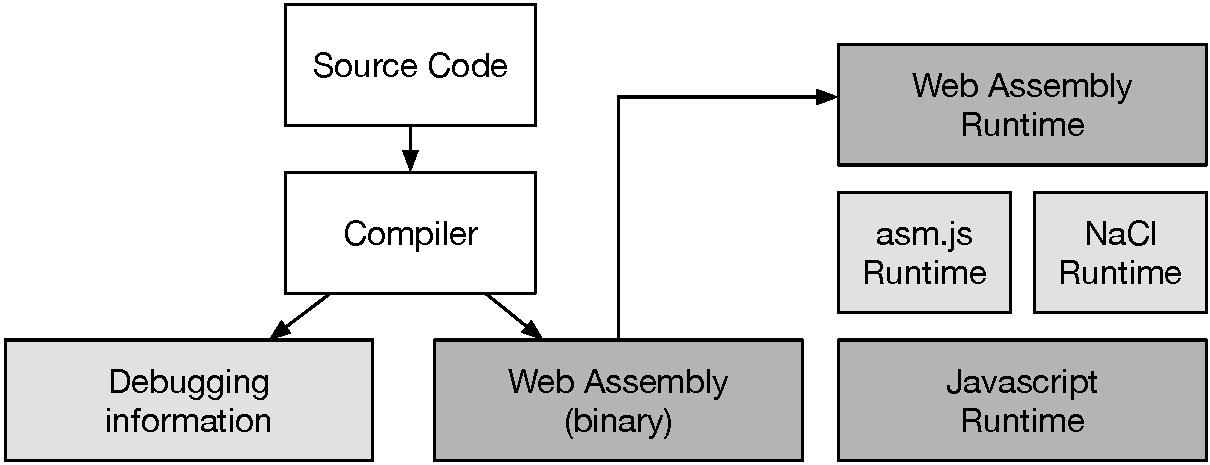
\includegraphics[width=0.7\linewidth]{imgs/wasm}
  \caption{WebAssembly 原型图}
  \label{fig:wasm}
\end{figure}

目前业界对于在浏览器中运行原生代码的解决方案,是综合了 Firefox 和 Chrome 浏览器两种思路而产生的。其主要借鉴了 asm.js 的思想,因此被称为 WebAssembly。如图 \ref{fig:wasm} 所示,WebAssembly 通过将原生代码编译为一种特殊的中间格式,然后在浏览器中执行编译产生的中间代码。WebAssembly 希望能够将运行时建立在 asm.js 和 Native Client 的抽象之上。目前 WebAssembly 已经支持将中间代码转换为 asm.js 来运行。这一方案是由 Firefox 的 asm.js 团队和 Chrome 的 Native Client 团队一起开发的,Native Client 团队因为其安全方面的特长,因此主要负责 WebAssembly 的安全与隔离。

WebAssembly 是以后 Web 发展的新趋势,也得到了谷歌、微软、苹果等公司的大力支持,以及 Javascript 之父 Brendan Eich 的背书。而 WebAssembly 目前还处于初级阶段,这其中自然存在一些安全问题。包括从编译器的代码生成环节,如何保证生成的代码是与原本的代码逻辑等价的;到在浏览器中运行时,如何安全地实现如同 Native Client 中原生代码与 Javascript 代码之间的交互,等等。这将是今后安全领域有一个新的研究点。这其中的问题未必能单独依靠沙箱技术来独立解决,由 Native Client 可知,现在的安全研究越来越多地涉及到多种技术的综合,WebAssembly 与编译器安全、操作系统安全、沙箱等等技术都有相关性。

% 研究点:移动端沙箱(Deprecated)

Capability作为另一种安全哲学,支持了细粒度的AC,其实可以被应用在很多地方。其在内核层面的实现,由于技术限制以及编程难度,并没有被商业OS们所真正采纳。而Capsicum作为其主要的内核实现,被纳入在FreeBSD 9中,并成为了Chromium在FreeBSD上的主要安全基础。可见,如何更好地权衡开销与性能,它在系统层面还有很长的路要走。退而求其次,capability-oriented programming则应运而生,即在程序设计层面应用Capability的安全哲学,其在程序设计上提出了相应的规范和要求,并得到了一定程度的认可和应用:OpenSSH, Apple's Security Server都遵循了这样的设计思路。也正因为如此,我们认为capability是三种沙箱技术中最具有实际的借鉴意义的。
